\begin{doublespace}
A Computer Aided Design (CAD) program is a type of computer software that aids in the design of mechanical systems. The CAD program that is used in this project is SolidWorks (\cite{dassault_systemes_3d_2021}). SolidWorks provides a graphical user interface (GUI) to assist in design, allowing its users to easily add and manipulate objects. Designs from SolidWorks can be exported to an stereolithography (STL) file which can later be 3D printed into real-life objects.

Before CAD programs existed, engineers and designers would design systems by hand. For most basic things this is fine. However, when designing complex systems, such as gear trains, this can become unrealistic. It is hard to draw three-dimensional objects on paper, and there are many calculations required which a computer can do in a fraction of the time a human can. With the invention of CAD software, such as SolidWorks, this design time was significantly reduced, but designing a gear train can still take hours, even for simple trains. If a mistake is found at the beginning of a gear train, the entire train needs to be fixed, adding much more time to the design.

This is the problem that a previous MQP team attempted to solve. They created a program with a simplified GUI which allows users to type in the gear information, then send it to SolidWorks to be generated automatically (\cite{holman_automated_2018}). A screenshot of the program can be seen in Figure~\ref{fig:old_gear_system}. This program greatly simplifies gear design. The users can create a design on paper, then enter the data points the program requires. Once they click "Generate in SolidWorks", the design is sent to SolidWorks and a CAD model is created automatically. This can save a designer many hours when they need to create a gear train.

\begin{figure}[htbp]
    \centering
    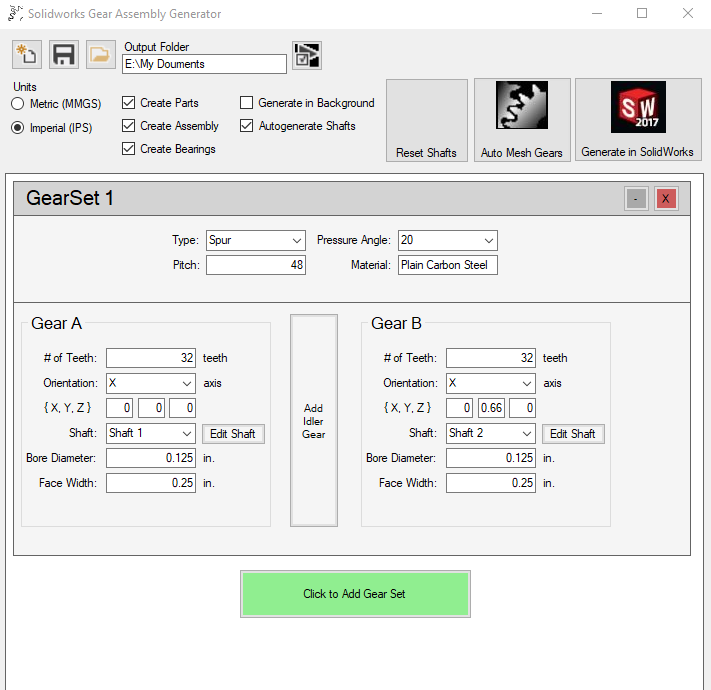
\includegraphics[width=\textwidth]{images/old_gear_system.png}
    \caption{Previous MQP gear design software.}
    \label{fig:old_gear_system}
\end{figure}

This program has many shortcomings and many places where it can be improved, as described in more detail in Chapter~\ref{sec:req}. One of the main goals of this project is to convert the software to the Windows Presentation Foundation (WPF) framework from Windows Forms. Windows Forms was the main graphical framework for .NET languages in the past, but Microsoft has ended support for it in favor of WPF (\cite{allen_wpf_2014}). With many new developers learning WPF instead of Windows Forms, it is important that the software be scalable and maintainable in the future by new developers. Additionally, WPF continues to receive updates by Microsoft, so new features are always available to add to the software if needed. In addition to updating the framework, other changes needed to be made to the software, including bug and UI fixes (according to our user studies, see Chapter~\ref{sec:eval}).

After creating our program, \emph{GearTrain}, based on comments about the old system, two more user studies were run on our system. In general, most participants found GearTrain easier to use than the old system, as explained in Chapter~\ref{sec:eval}. The whole purpose of GearTrain is to make designing gear trains as easy as possible. By focusing on Human Computer Interaction (HCI) principles and user interaction, we were able to create a system that is very easy to use while still being able to create complex gear train designs.

Chapter~\ref{sec:req} describes the problem that this project will try to solve in more detail, as well as the requirements. Chapter~\ref{sec:lit} describes some of the related work to our project and the various resources we used. Chapter~\ref{sec:method} describes the steps taken to complete the project and the methods used. Chapter~\ref{sec:design_ui} explains the design decisions made for the user interface design, while Chapter~\ref{sec:design_sys} discusses the design of the system internally and the rationale for some of these decisions. Chapter~\ref{sec:data} contains the analysis of the data for our user studies, including some raw results. Chapter~\ref{sec:eval} discusses the significance and conclusions of the studies that were done and how the results were applied to our project. Finally, Chapter~\ref{sec:concl} concludes this project.

\end{doublespace}